\chapter{Factoring Polynomials}

We factor a polynomial into two or more polynomials of lower
degree. For example, let's say that you wanted to factor
$5x^3 - 45x$. You would note that you can factor out $5x$ from every term. Thus,
\begin{equation*}
5x^3 - 45x = (5x)(x^2 - 9)
\end{equation*}
You might notice that the second factor looks like the difference of squares, so
\begin{equation*}
5x^3 - 45x = (5x)(x + 3)(x - 3)
\end{equation*}
That is as far as we can factorize this polynomial.\index{factoring polynomials}

Why do we care? The factors make it easy to find the roots of the
polynomial. This polynomial evaluates to zero if and only if at least
one of the factors is zero. Here, we see that
\begin{itemize}
\item The factor $(5x)$ is zero when $x$ is zero.
\item The factor $(x + 3)$ is zero when $x$ is -3.
\item The factor$(x - 3)$ is zero when $x$ is 3.
\end{itemize}
So, looking at the factorization, you can see
that $5x^3 - 45x$ is zero when $x$ is 0, -3, or 3. 

This is a graph of that polynomial with its roots circled:

\begin{figure}[htbp]
    \centering
    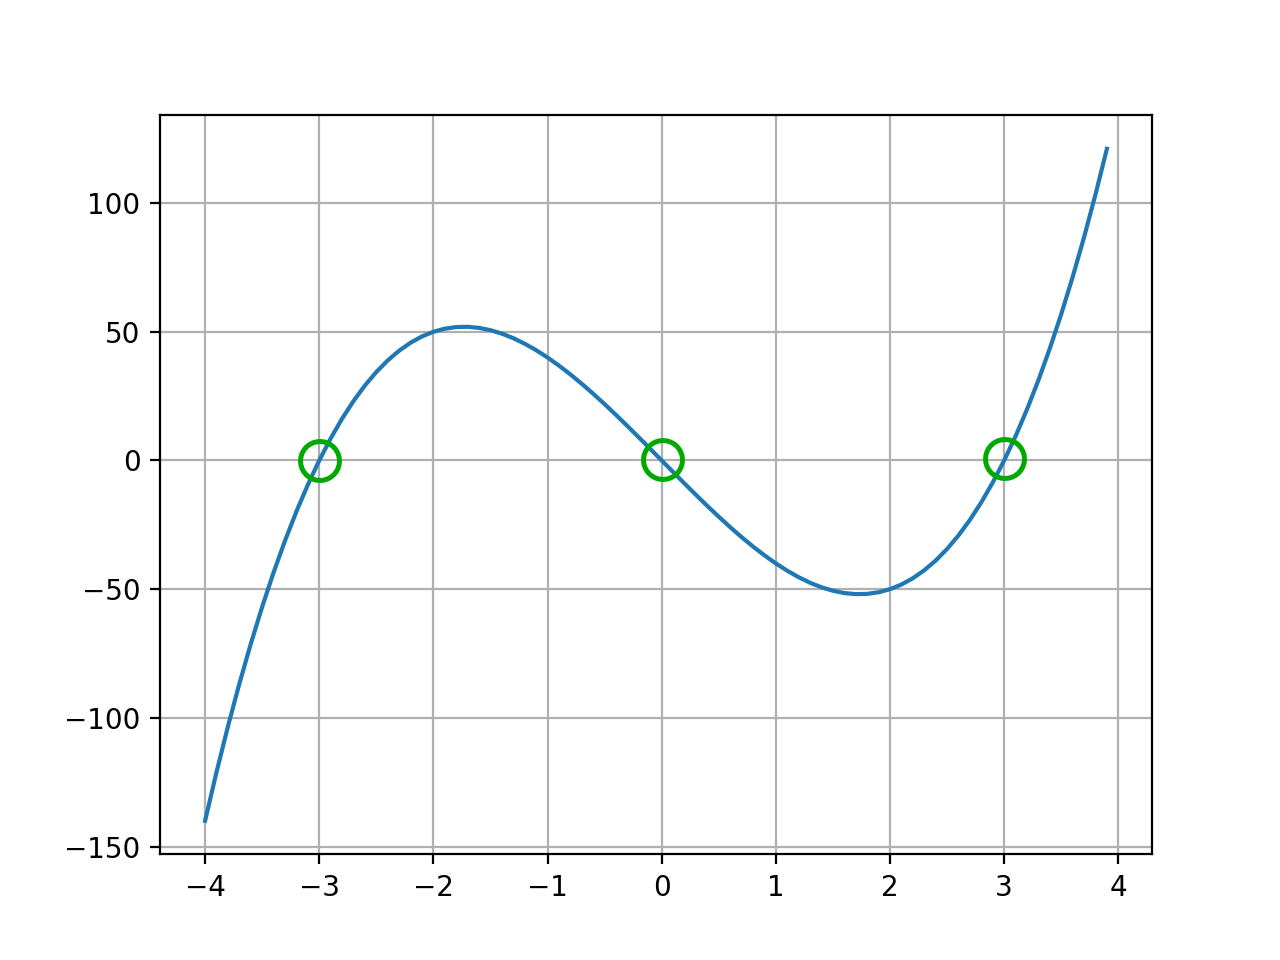
\includegraphics{factor4roots.png}
    \caption{Factoring for roots makes it easier to find the roots rather than in expanded form.}
    \label{fig:factor4roots}
\end{figure}

\section{How to factor polynomials}

The first step when you are trying to factor a polynomial is to find
the greatest common divisor for all the terms, then pull that out. In
this case, the greatest common divisor will also be a monomial. Its
degree is the least of the degrees of the terms, its coefficient will
be the greatest common divisor of the coefficients of the terms.

For example, what can you pull out of this polynomial?
\begin{equation*}
12x^100 + 30x^31 + 42x^17
\end{equation*}
The greatest common divisor of the coefficients (12, 30, and 42) is 6.  The least of the degrees of terms (100, 31, and 17) is 17.  So, you can pull out $6x^17$:
\begin{equation*}
12x^100 + 30x^31 + 42x^17 = (6x^17)(2x^83 + 5x^14 + 7)
\end{equation*}

\begin{Exercise}[title={Factoring out the GCD monomial}, label=gcdmonomial]
FIXME Exercise here
\end{Exercise}
\begin{Answer}[ref=gcdmonomial]
  
\end{Answer}

So, now you have the product of a monomial and a polynomial. If you
are lucky, the polynomial part looks familiar, like the difference of
squares or a row from Pascal's triangle.

Often, you are trying factor a quadratic like $x^2 + 5x + 6$ in a pair
of binomials. In this case, the result would be $(x + 3)(x + 2)$. Let's check that:
\begin{equation*}
  (x + 3)(x + 2) = (x)(x) + (3)(x) + (2)(x) + (3)(2) = x^2 + 5x + 6
\end{equation*}
Notice that 3 and 2 multiply to 6 and add to 5. If you were trying to
factor $x^2 + 5x + 6$, you would ask yourself''What are two numbers that
when multiplied equal 6 and when added equal 5?'' And you might
guess wrong a couple of times. For example, you might say to youself,
``Well, 6 times 1 is 6. Maybe those work. But 6 and 1 add 7. So those
don't work.''

Solving these sorts of problems are like solving a Sudoku puzzle. You
try things and realize they are wrong, so you backtrack and try
something else.

The numbers are sometimes negative. For example, $x^2 + 3x - 10$ factors into $(x + 5)(x - 2)$.

\begin{Exercise}[title={Factoring quadratics}, label=factorquadratics]
  
\end{Exercise}
\begin{Answer}[ref=factorquadratics]
  
\end{Answer}
